\section{Volunteer Trials} \label{sec:develop_trials}
    This works’ field research is composed of, as determined before, user trials in a controlled environment with the goal of finding and collecting insight in regard to the usage of Cultural Awareness as the primary solution for the issue of user spontaneity and adaptability, and the hypotheses stated within the Goals section\ref{sec:intro_goals}.\\
    The planning surrounding the user trials was carried out with the intent of facilitating the forms of techniques employed in data collection useful for evaluation, those being observation data and user opinion data. These are performed concurrently to differing degrees of focus in accordance to different parts of each trial. These parts of a trial roughly follow the directions of the outline provided earlier in the section on HCI Evaluation\ref{sec:hci_definition_goals}, however, they will be detailed further in the following sections and an overview provided is provided in image \ref{fig:FigureTrialSections}.
    
    \begin{figure}[ht]
        \hspace*{-1cm}
        \centering                                                
        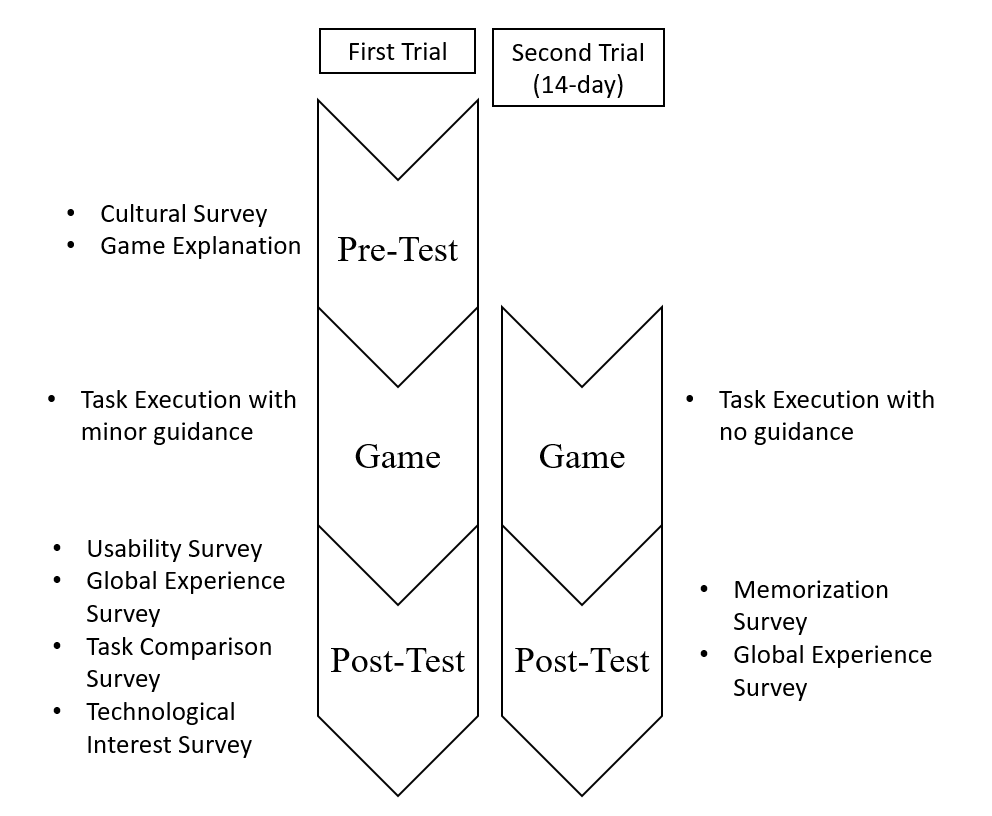
\includegraphics[width=.9\paperwidth]{figures/TrialSections.png}
        \caption{\label{fig:FigureTrialSections}Overview of User Trial's Sections.}               
    \end{figure}
    
    \subsection{Pre-Test} \label{sec:develop_trials_pre}
    The pre-test is the initial part of the trial, and it matches up roughly to the Introduction and Warm-Up phases of a field study plan. Users are introduced to the controlled environments, the room and equipment, and are initially asked for their demographic data and some first impressions and some very basic questions, such as, if they have knowledge of the apparatus used in gesture detection presented, the Leap Motion. They are also allowed to test out the Leap Motion’s diagnostic visualizer for up to 30 seconds just to get a rough idea of its function.\\
    However, there’s two bigger main components to the Pre-test after the initial introduction. A Cultural Survey and a Game Explanation.\\
    The Cultural Survey is done before any information about the game is given to the volunteer. They are presented with a simple black text on white background slide show containing several snippets indicating a different message. Each message represents one of the game’s task, and the volunteer is tasked with performing the gestures they feel best describe that action or message. The main objective of this exercise is checking if the user performs a majority of the same moves as the ones the Cultural Group uses during the game. This is a requirement of this work as a counter-measure against certain potentially erroneous assumptions made during development, such as, most directly, the choice of gestures the tasks use. Should the majority of users name the same gestures as the Cultural Group, this helps pre-emptively validate the game as a cultural experience. Should the majority name a specific different gesture, that should, conversely, invalidate that task for result-checking.\\
    The Game Explanation happens right afterwards. Here, the volunteers are shown a depiction of the in-game tasks they’ll have to perform, in the same order as the messages they just read through, both in the slide show and with a separate physical document. There are different explanations for the cultural and non-cultural group, however, those difference are never stated. The volunteers are given instructions on how to perform the tasks, as well as the differences between the Interaction Spaces and the method by which the game progresses. Finally, they’re asked if they understand the purpose of the gesture used in the task. Their comments and understanding are written down and recorded. Here the non-cultural users are implicitly given an opportunity to name their preference for one of the tasks they performed previously.\\
  
    \subsection{Game Observation} \label{sec:develop_trials_game}
    Following the explanation of the game, the volunteers are ready to play the game proper. Here, they are asked to perform the game fully. The volunteers are given a few more pointers to aid them on the way, mainly with getting used with movement, but are never outright given the actual gestures required for a task. They are also prompted for help if they appear to have difficulties at certain steps but are only given it if they accept or request it.\\
    Any special observation is recorded, priority given to unexpected displays of frustration or amusement. But some aspects of observing the user are most important for this segment. The Time Elapsed, the Number of User Errors, if Help was Required, and if the Correct Gesture was actually performed. These are likely to provide the most qualitative insight and are discernible enough to make an immersion scoring out of, and as such, the protocol developed for the trial is to document these values for every single task and every single volunteer, with both help from recordings (when permitted) and the game’s own logging of each task.\\

    \subsection{Post-Test} \label{sec:develop_trials_post}
    After the game is completed, the volunteer is given a moment to rest and then they’re asked to go over a questionnaire and answer it. This is closely related to the Cool-Off period of a field research and is the adequate time to investigate questions in the form of a survey. Volunteers aren’t asked to answer on their own, but rather, all of the questions are read out to the users and they’re made clearly aware of what each question is asking, slowing down the pace between questions if they’re answering too fast, and prodding for certainties in responses when a bout of indecision arises.\\
    There are three parts to the post-test questionnaire. The first part is a usability survey. Since the game was rewritten from scratch, it stands that its usability is still unproven and must be evaluated, however, the real reasoning behind making this investigation is that many aspects of usability have crossover with immersion and satisfaction signifiers. Thus, this is an insightful exercise towards the goals of this work and helps frame the way by which further questioning will be administered. The questions presented in the first part are adapted from the System Usability Scale. All scores of the scale are present and answers are scaled such as a 0-100 usability score is possible. Some other satisfaction-related questions were dropped here, particularly, that of the least enjoyable or most concerning aspect of the game, to ensure users don’t leave out details about their frustrations.\\ 
    The second part of the questionnaire goes over every Task and asks two questions on a scale for each of the gestures. The two aspects are surveyed are the ease of the gesture, and the natural fit of the gesture for the task. Since the users may find different interpretations for the scale, this one is meant to be taken as a comparative measure between each of the gestures, scoring them in terms of ‘below than ideal’. This should provide some final insights into the choice of gestures and their applicability for the task, but moreover, should provide a focal point of comparison between the Cultural and Non-Cultural groups.\\
    The third part is short, and merely looks into the volunteer’s experience with computers on their daily lives and their interest and pre-existing capabilities using other natural systems. This was a concern that could arise if groups of volunteers appeared to have vastly different expectations and performances between one another.\\
    
    \subsection{Second Trial} \label{sec:develop_trials_second}
    After performing the trial, the users are thanked and allowed to depart. However, their contribution isn’t over at this point. Given that one aspect of the proposed benefits to the shamanic interface approach has a large emphasis on memorization of commands, these have to be tested after a delay of time with no exposure to the system. All participants are therefore asked to come back and fulfil a second follow-up trial after a period of 14 days minimum. The goal here is to assess if their memory of the content still matches the actual experience. The second trial has two parts, first the volunteers perform the game again, and then they’re given a new post-game questionnaire.\\
    Absolutely nothing is changed with the game builds themselves, as the experience must remain consistent with the previous. Also, the same indicators have primary focus during observation, those being Number of User Error and so on. However, a small difference is with the protocol is that time, the users are not given any of the previous helpful pointers and are not prompted on their need of help if they’re seen struggling. The players must request help themselves if they appear to struggle and are allowed to proceed with failure if they don’t remember the task gesture but are certain of an erroneous one. This compels users to rely only on their own recollection of the solutions and in taking their time, rather than rely on communication with the researcher. The benefit of taking this approach is that it highlights their confidence on the gestures given without it needing to be taken in survey. To that end, the users are also not corrected on gestures until the second trial is over and they’re no longer under observation.\\
    The second post-game questionnaire is different from the first trials. This questionnaire has two parts. The first goes over every task and surveys users on their ease remembering each gesture. This is, again, meant to highlight a difference between each of the two Cultural groups, as the Non-cultural is predicted to mention greater barrier against the Cultural group. Additionally, there may also be a significant disparity between self-confidence and erroneous resolution of gestures in this aspect between the two groups, which may be of interest to record. As for the second part of the questionnaire, instead of focusing mostly on usability like the previous, this time, users are prompted over categories of experiential quality indicators. They’re asked about the impact, agreement and value of several aspects of the experience which they may rate on a 5-point scale between Strong Disagreement and Strong Agreement, although the majority just kept to simple a binary dimension between Yes and No or Good and Not Good answers. Listing the categories, their affective expectations, their feelings, their self-consciousness, the repeatability and their willingness to share with and recommend to others, their thoughts on the applicability and usability of the type of experience among different groups of people, the technological quality of the experience, and sense making and meaningful feedback.\\